% --- Template for thesis / report with tktltiki2 class ---
%
% last updated 2013/02/15 for tkltiki2 v1.02

\documentclass[finnish]{tktltiki2}

  % tktltiki2 automatically loads babel, so you can simply
  % give the language parameter (e.g. finnish, swedish, english, british) as
  % a parameter for the class: \documentclass[finnish]{tktltiki2}.
  % The information on title and abstract is generated automatically depending on
  % the language, see below if you need to change any of these manually.
  %
  % Class options:
  % - grading                 -- Print labels for grading information on the front page.
  % - disablelastpagecounter  -- Disables the automatic generation of page number information
  %                              in the abstract. See also \numberofpagesinformation{} command below.
  %
  % The class also respects the following options of article class:
  %   10pt, 11pt, 12pt, final, draft, oneside, twoside,
  %   openright, openany, onecolumn, twocolumn, leqno, fleqn
  %
  % The default font size is 11pt. The paper size used is A4, other sizes are not supported.
  %
  % rubber: module pdftex

  % --- General packages ---

  \usepackage[utf8]{inputenc}
  \usepackage[T1]{fontenc}
  \usepackage{lmodern}
  \usepackage{microtype}
  \usepackage{amsfonts,amsmath,amssymb,amsthm,booktabs,color,enumitem,graphicx}
  \usepackage[pdftex,hidelinks]{hyperref}

  \graphicspath{{images/}}

  % Automaticall set the PDF metadata fields
  \makeatletter
  \AtBeginDocument{\hypersetup{pdftitle = {\@title}, pdfauthor = {\@author}}}
  \makeatother

  % --- Language-related settings ---
  %
  % these should be modified according to your language

  % babelbib for non-english bibliography using bibtex
  \usepackage[fixlanguage]{babelbib}
  \selectbiblanguage{finnish}

  % add bibliography to the table of contents
  \usepackage[nottoc]{tocbibind}
  % tocbibind renames the bibliography, use the following to change it back
  \settocbibname{Lähteet}

  % --- Theorem environment definitions ---

  \newtheorem{lau}{Lause}
  \newtheorem{lem}[lau]{Lemma}
  \newtheorem{kor}[lau]{Korollaari}

  \theoremstyle{definition}
  \newtheorem{maar}[lau]{Määritelmä}
  \newtheorem{ong}{Ongelma}
  \newtheorem{alg}[lau]{Algoritmi}
  \newtheorem{esim}[lau]{Esimerkki}

  \theoremstyle{remark}
  \newtheorem*{huom}{Huomautus}


  % --- tktltiki2 options ---
  %
  % The following commands define the information used to generate title and
  % abstract pages. The following entries should be always specified:

  \title{Konvolutionaaliset neuroverkot}
  \author{Teemu Sarapisto}
  \date{\today}
  \level{Kandidaatintutkielma}
  \abstract{
  Viimeisen hieman yli kymmenen vuoden aikana voidaan sanoa keinotekoisten neuroverkkojen ja syväoppimisen tehneen läpimurron. Syväoppimisen voidaan katsoa syntyneen jo 40-luvulla, mutta laajamittaiseen sovelluskäyttöön se on tullut vasta viime vuosina, kun sekä riittävä määrä luokiteltua dataa, että riittävästi prosessointitehoa on tullut helposti saataville. Myös algoritmipuolella tapahtuneet edistykset ovat edesauttaneet läpimurtoa. Aikaisemmin koneoppimisen alalla haasteelliseksi osoittautuneissa sovelluskohteissa kuten kuvien sekä puheen sisällön tunnistamisessa keinotekoiset neuroverkot ovat osoittautuneet toistaiseksi ylivoimaisesti parhaiten toimiviksi ratkaisuiksi.
  
  Neuroverkkojen opetuksessa tärkeimpiä menetelmiä ovat gradienttimenetelmä ja takaisinvirtausalgoritmi
  
  Konvolutionaaliset neuroverkot ovat eräänlaisia neuroverkkoja jotka soveltuvat hyvin kuvien ja muiden paikallisuudesta hyötyvien syötteiden käsittelyyn}

  % The following can be used to specify keywords and classification of the paper:

  \keywords{neuroverkot, neuroverkkojen harjoittaminen, kuvien luokittelu}

  % classification according to ACM Computing Classification System (http://www.acm.org/about/class/)
  % This is probably mostly relevant for computer scientists
  % uncomment the following; contents of \classification will be printed under the abstract with a title
  % "ACM Computing Classification System (CCS):"
  % \classification{}

  % If the automatic page number counting is not working as desired in your case,
  % uncomment the following to manually set the number of pages displayed in the abstract page:
  %
  % \numberofpagesinformation{16 sivua + 10 sivua liitteissä}
  %
  % If you are not a computer scientist, you will want to uncomment the following by hand and specify
  % your department, faculty and subject by hand:
  %
  % \faculty{Matemaattis-luonnontieteellinen}
  % \department{Tietojenkäsittelytieteen laitos}
  % \subject{Tietojenkäsittelytiede}
  %
  % If you are not from the University of Helsinki, then you will most likely want to set these also:
  %
  % \university{Helsingin Yliopisto}
  % \universitylong{HELSINGIN YLIOPISTO --- HELSINGFORS UNIVERSITET --- UNIVERSITY OF HELSINKI} % displayed on the top of the abstract page
  % \city{Helsinki}
  %


  \begin{document}

  % --- Front matter ---

  \frontmatter      % roman page numbering for front matter

  \maketitle        % title page
  \makeabstract     % abstract page

  \tableofcontents  % table of contents

  % --- Main matter ---

  \mainmatter       % clear page, start arabic page numbering

  \section{Johdanto}
   Syväoppimisen historia ulottuu 1940-luvulle asti \cite{Goodfellow-et-al-2016}, jolloin kybernetiikan tutkimuksen myötä McCulloch ja Pitts kehittivät mukaansa nimetyn McCulloch-Pitts neuronin, tarkoituksenaan luoda matemaattinen malli, jolla kuvailla biologista aivoissa tapahtuvaa oppimista \cite{mcculloch1943logical}. Heidän kehittelemällään lineaarisella mallilla oli mahdollista tunnistaa kahden syötekategorian välillä kategoriat määrittelevien painotuksien avulla ihmisen joutuessa määrittelemään nämä painot. Vasta 1950-luvulla kehitettiin ensimmäinen malli joka pystyi oppimaan syötekategorioita kuvaavat painotukset niistä annettujen esimerkkien perusteella, niin kutsuttu perseptroni \cite{rosenblatt1957perceptron}.

  Kiinnostus kybernetiikkaan hiipui 1960-luvun aikana, jonka jälkeen merkittävää kehitystä tapahtui seuraavan kerran vasta 80-90-luvulla konnektionismin tuodessa neuroverkkomallit takaisin suosioon. Yksi tärkeimmistä näihin aikoihin tapahtuneista kehityksistä syväoppimisen kannalta oli, kun takaisinvirtausalgoritmin (backpropagation) keksittiin 1986 soveltuvan monikerroksisten neuroverkkojen tehokkaaseen harjoittamiseen \cite{Rumelhart-1986-back-prop}.

  90-luvun puolivälin jälkeen syväoppiminen eli jälleen hiljaiseloa vuoteen 2006 asti, jonka jälkeen se on ollut jatkuvasti pinnalla tähän päivään asti. Geoffrey Hinton osoitti tällöin syvien uskomusverkkojen (deep belief network) olevan harjoitettavissa tehokkaasti tasoittain ja muut tutkimusryhmät yleistivät tämän harjoitustavan muille syville keinotekoisille neuroverkoille \cite{Hinton-et-al-06}. Näiden tutkimuksien myötä syväoppiminen terminä alkoi yleistyä, termin käytön tarkoituksena korostaa aikaisempaa syvempien verkkojen harjoitettavissa olemista.

  Lopullinen syväoppimisen läpimurto tapahtui vuonna 2012 kun suurimman kuvista objektien tunnistamisen kilpailun, ImageNet Large Scale Visual Recognition Challengen (ILSVRC), voitti ensimmäistä kertaa syvä konvolutionaalinen neuroverkko \cite{KSHimagenet2012}. Voitto tapahtui myös huomattavalla erolla toisen sijan saavuttaneeseen sekä aikaisempien vuosien voittajiin. Tämän jälkeen kilpailun on joka vuosi voittanut syvä konvoluutioverkko, ja nykyään neuroverkot pärjäävät kyseisessä varsin rajoitetussa tunnistamistehtävässä ihmistä paremmin.

  Nykyään ihmisille monimutkaisissakin tehtävissä pärjäävät oppimisalgoritmit ovat pääasiassa samoja kuin jo 80-luvulla keksityt. Jonkin verran muutoksia silloisiin algoritmeihin on kuitenkin tehty, erityisesti syvien verkkorakenteiden harjoittamista helpottavina yksinkertaistuksina. Selkeästi suurin syy syväoppimisen vasta äskettäin tärkeäksi muuttumiseen on kuitenkin yhteiskunnan digitalisoitumisen myötä merkittävästi kasvanut helposti saatavilla olevan luokitellun datan määrä, sekä valtavasti kasvanut laskentakapasiteetti, jotka olivat edellytyksiä algoritmien mielekkäälle käyttämiselle \cite{Goodfellow-et-al-2016}.

  Esimerkkinä tarvittavan harjoitusdatan määrästä konvolutionaalisten neuroverkkojen harjoittamiseen kuvien luokittelua varten toimii yleensä tuhansia ellei jopa miljoonia kuvien sisällön perusteella etukäteen luokiteltuja kuvia. Esimerkiksi ILSVRC-kilpailun harjoitusdatana käytössä oleva ImageNet sisältää yli 14 miljoonaa luokiteltua kuvaa \cite{imagenet-website}. Kuvien sisällön tunnistamisen lisäksi syväoppiminen on osoittautunut erittäin hyödylliseksi useissa aikaisemmin haasteellisiksi osoittautuneissa sovelluskohteissa, kuten puheentunnistuksessa \cite{abdel2012applying}, liikennemerkkien luokittelussa \cite{sermanet2011traffic}, sekä jalankulkijoiden tunnistamisessa \cite{szarvas2005pedestrian}.

  Ensin käydään läpi yleisiä keinotekoisten neuroverkkojen piirteitä, kuten yksittäisten neuronien ja eteenpäinsyöttävien neuroverkkojen rakennetta. Tämän jälkeen selitetään kuinka neuroverkkoja harjoitetaan harjoitusaineiston avulla takaisinvirtausalgoritmia ja gradienttimenetelmää hyödyntäen. Lopuksi käydään läpi miten konvolutionaaliset neuroverkot eroavat muista neuroverkoista ja mitä sovelluksia niille löytyy.

  \section{Neuroverkkojen rakenne}
  \subsection{Keinotekoinen neuroni}
    \label{chap:artificial-neuron}

    %TODO: lähdeviitteet! 
    TODO: Pitäisikö tässä tai johdannon lopussa mainita, että rakenneosiot ovat Neural Networks and Deep Learning kirjasta \cite{Nielsen-neural} peräisin ja ei lisätä citeä joka lauseen loppuun? 

    Biologisista vaikuttimistaan huolimatta keinotekoiset neuronit ovat käytännössä (TODO: selitä pelkästään tekstimuodossa re: palaute)

     $$ x_1, x_2, ..., x_n \mapsto \Sigma w_i x_i \mapsto f(\Sigma w_i x_i + b) $$

    kaltaisia matemaattisia funktioita. Ne ottavat vastaan yhden tai useampia syötteitä $x_1$, $x_2$, ..., $x_n$, joista kullekin on asetettu jokin painoarvo $w_i$. Syötteiden ja painotuksien tulojen summa $\Sigma x_i w_i$ annetaan parametrina aktivaatiofunktiolle $f$ ja tämän funktion arvo toimii neuronin lopullisena ulostuloarvona. Toisinaan käytetään myös taipumusvakiota (bias) $b$, joka lisätään syötteiden ja painotuksien tulojen summaan, tarkoituksena säätää neuronin ulostuloarvoja painotuksista riippumatta \cite{Nielsen-neural}.

    50-luvulla kehitetyn perseptronin, joka oli ensimmäinen tällainen neuroni, syötteet ja ulostuloarvot ovat binäärisiä ja aktivaatiofunktio muotoa

    \begin{equation}
      f(\Sigma w_i x_i + b)
      \begin{cases}
        0\; \text{jos} \; \Sigma x_i w_i + b \leq 0 \\
        1\; \text{jos} \; \Sigma x_i w_i + b > 0. \\
      \end{cases}
      \label{eq:perceptron}
    \end{equation}

    Yksittäisen neuronin tasolla neuronien oppiminen tapahtuu syötteiden painotuksien ja taipumusarvon muuttumisen kautta. Perseptroneja käytettäessä törmätään kuitenkin usein ongelmaan, jossa yksi pieni muutos painotuksissa tai taipumusarvossa johtaa ulostuloarvon vaihtumiseen, joka saattaa aiheuttaa suuria muutoksia ulostuloarvoissa myös koko neuroverkon tasolla. Usein halutaan hienovaraisempia muutoksia ja tällöin käytetään neuroneita joiden syöte- ja paluuarvot voivat olla myös mitä vain reaalilukuja nollan ja yhden väliltä. Esimerkiksi yksi tällainen laajalti käytössä oleva neuroni on sigmoidinen neuroni, jonka aktivaatiofunktiona toimii sigmoidinen funktio.

  %kappaleessa 3 rojanista hyvää juttua \cite{Rojas96}

  %http://neuralnetworksanddeeplearning.com/chap1.html keksi parempi lähde
  % oliko varmasti 50-luvulla?

  \subsection{Keinotekoisten neuroverkkojen rakenne}

  \begin{figure}[h]
  \centering
  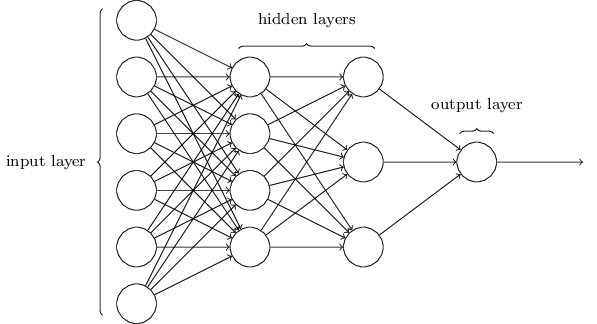
\includegraphics[scale=0.5]{basic-neuralnet}
  \caption{Tyypillinen neuroverkon rakenne, jossa kaksi piilokerrosta \cite{Nielsen-neural}}
  \label{pic:neuralnet}
  \end{figure}

  Yksinkertaisimman verkkorakenteen omaavat eteenpäinsyöttävät neuroverkot muodostetaan tasoittain, jossa jokaisen verkon tason neuronit saavat syötteenään niitä edeltävän tason neuroneiden ulostuloarvot. Poikkeuksena ensimmäinen taso (kuvassa vasemmanpuoleisimpana), joihin verkon syöte koodataan. Esimerkiksi haluttaessa syöttää 64x64 kuva neuroverkolle voidaan syötekerroksena käyttää 64x64 neuronin kerrosta, johon kuvan pikselien väriarvot koodataan. Neuroverkon laskennan lopputuloksena toimii verkon viimeisen tason neuroneiden ulostuloarvot.

  Vaikka syväoppimista voidaan harjoittaa myös muutoin kuin keinotekoisilla neuroverkoilla, neuroverkkojen tapauksessa termillä viitataan neuroverkkojen piilokerroksiin ja niiden määrään. Kasvattamalla neuroverkkotasojen sekä tasoissa olevien neuronien määrää neuroverkoilla voidaan mallintaa entistä monimutkaisempia funktioita.

  \section{Neuroverkkojen harjoittaminen}
    \label{chap:neural-training}

  % mitä tahansa jatkuvia $R^n$ kompaktien aliavaruuksien funktioita, 
    Eteenpäinsyöttävien neuroverkkojen joissa on yksi piilokerros jossa on tarpeeksi neuroneita on todistettu pystyvän mallintamaan mitä tahansa avaruuden $R^n$ kompakteilla osajoukoilla määriteltyjä jatkuvia funktioita, kunhan tarpeeksi laskentaresursseja on käytettävissä \cite{multilayer-feedforward-universal-approximators}. Neuroverkkojen harjoittamisen voidaan sanoa olevan neuroverkon tekemän virheen minimointia sen approksimoidessa jotakin funktiota.

  Tätä neuroverkon tekemän virheen määrää voidaan mitata virhefunktion (error function) avulla. Usein käytetään neliöllistä virhefunktiota
  \begin{equation}
    E(x) = \frac{1}{2} \sum_{i=1}^{N} \| y(x_i) - z_i \|^2
    \label{eq:error-function}
  \end{equation}
  jossa $y(x_i)$ on neuroverkon tulos syötteellä $x_i$, $z_i$ on jonkin harjoitusaineiston yksikön $i$:s jäsen, ja $N$ syötteiden määrä.

  %% TOOO: Mainitse että koko harjoitusdatalle lasketaan yksittäisten kierroksien virhefunktioiden arvoista keskiarvo. Smaa pätee painojen ja taipumusvakioiden derivaatoille, niistä otetaan vain keskiarvo. Tästä sais kokonaisen kappaleen lisää? Stokastisen gradienttimenetelmän kohdalla kylläkin mainitaan asiasta lyhyesti

  % The reason we need this assumption is because what backpropagation actually lets us do is compute the partial derivatives  and  for a single training example. We then recover  and  by averaging over training examples.


  \subsection{Gradienttimenetelmä ja takaisinvirtausalgoritmi}
  Gradienttimenetelmä (gradient descent) on numeerinen menetelmä joka toimii minkä tahansa derivoituvan funktion lokaalien minimien etsintään. Käytännössä kuitenkin yleensä riittää, että funktiot ovat suurimmilta osin derivoituvia. Neuroverkkojen yhteydessä gradienttimenetelmä toimii valittaessa neuronien aktivaatiofunktioksi pääosin derivoituvia funktioita, jolloin myös koko neuroverkon tuottamat arvot ja siten virhefunktio ovat derivoituvia. Gradientti kertoo mihin suuntaan funktion arvo laskee nopeimmin, joten kuljettaessa iteratiivisesti tähän suuntaan, kunnes gradientti on tarpeeksi pieni, päädytään lähelle lokaalia minimiä.

  Takaisinvirtausalgoritmilla voidaan laskea virhefunktiolle osittaisderivaatta kunkin verkon painon suhteen. Osittaisderivaatoista voidaan muodostaa virhefunktiolle gradientti ja siten soveltaa gradienttimenetelmää. Virhefunktion osittaisderivaatan selvittämiseksi yksittäisen neuronien $n_i$ ja $n_j$ välillä olevan verkon painon $w_{ij}$ suhteen tarvitaan ensin välituloksena virhefunktion osittaisderivaatta neuronin $n_j$ kohdalla. 

  Neuroverkon voidaan ajatella olevan yhdistetty funktio sen neuroneiden funktioista, joten derivoimisessa voidaan soveltaa ketjusääntöä. Jotta virhefunktion arvot saadaan osaksi verkkoa, lisätään ulostulokerroksen jälkeen yksi näennäinen neuroni, joka ottaa ulostulokerroksen neuroneiden ulostulot syötteenään, ja laskee niiden perusteella virhefunktion arvon. Nyt virhefunktion derivaattojen laskentaan voidaan hyödyntää seuraavaksi esitettävää verkkomuotoista derivaatan ketjusäännön toteutusta. 
    
  \begin{figure}[h]
    \centering
    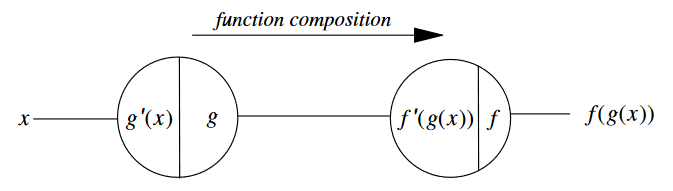
\includegraphics[scale=0.5]{function-composition}
    \caption{Ketjusääntö ja eteenpäinvirtaus kahden solmun verkossa \cite{Rojas96}}
    \label{pic:composition}
  \end{figure}

  Ketjusäännön mukainen derivointi suoritetaan kahdessa osassa, käyden verkko ensin läpi normaaliin suuntaan syötteistä ulostuloarvojen kautta virhefunktion arvoon, ja sen jälkeen takaperin. Takaisinvirtausalgoritmi on saanut nimensä tästä taaksepäin kulkemisesta, jossa virhefunktion arvojen voidaan ajatella virtaavan taaksepäin verkon loppupäästä.
  
  Eteenpäinsyöttövaiheessa jokaisen solmun kohdalla tallennetaan solmun toteuttaman funktion derivaatta. Kuvassa \ref{pic:composition} tämä tallennettava arvo näkyy palloina esitettyjen solmujen vasemmassa puoliskossa.

  \begin{figure}[h]
    \centering
    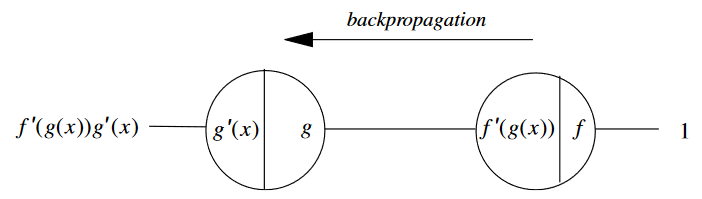
\includegraphics[scale=0.5]{backpropagation}
    \caption{Ketjusääntö ja takaisinvirtaus kahden solmun verkossa \cite{Rojas96}}
    \label{pic:backpropagation}
  \end{figure}

  Takaisinvirtausvaiheessa verkkoa kuljetaan takaperin aikaisempaan nähden. Takaisinvirtaus aloitetaan syöttämällä verkkoon numero yksi, kuljettaen tätä arvoa mukana solmulta toiselle, ja uuteen solmuun saavuttaessa kertomalla mukana kulkeva arvo solmuun tallennetulla, kuvassa \ref{pic:backpropagation} solmun vasemmalla puoliskolla näkyvällä arvolla. Näin lopulta esimerkin kahden solmun läpi kulkemisen jälkeen yhdistetty funktio $f(g(x))$ on saatu muotoon $f'(g(x))g'(x)$, joka on funktion $f(g(x))$ derivaatta. 

  Kuvaamalla virhefunktion derivaattaa neuronin $n_j$ kohdalla merkinnällä $\delta_j$ voidaan virhefunktion derivaatta suhteessa painoon $w_{ij}$ esittää muodossa 

    $$ \frac{\partial E}{\partial w_{ij}} = o_i\delta_j,$$

  jossa $o_i$ on neuronin $n_i$ ulostuloarvo.

  \begin{figure}[h]
    \centering
    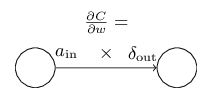
\includegraphics[scale=0.8]{cost-derivative}
    \caption{Virhefunktion derivaatta yksittäisen painon suhteen \cite{Nielsen-neural}. TODO: piirrä oma kuva omilla merkinnöillä}
    \label{pic:cost-weight-derivative}
  \end{figure}

  Virhefunktion arvon laskeminen jokaiselle syötteelle ja keskiarvon ottaminen ja tämän perusteella takaisinvirtausalgoritmin suorittaminen olisi erittäin raskasta kun syötteitä voi olla miljoonia kappaleita. Tämän takia käytetään yleensä stokastista gradienttimenetelmää, jossa virhefunktion keskiarvo lasketaan kaikkien syötteiden sijaan joukolle satunnaisesti valittuja syötteitä, ja ajetaan takaisinvirtausalgoritmi tämän tuloksen perusteella.

  \subsection{Ylisovitus ja sen ratkaiseminen}

  %Koneoppimisessa haaste ylisovitus
  Suuri haaste neuroverkkojen harjoittamisessa on ylisovitus (overfitting), jossa neuroverkon harjoittamisen jälkeen neuroverkko saa harjoitusaineistosta valituille syötteille pieniä arvoja virhefunktiosta, mutta uuden aineiston kanssa virhefunktio tuottaa suuria arvoja. Tällöin neuroverkon oppima malli vastaa harjoitusaineistoa liian tarkkaan, eikä pysty yleistämään harjoitusaineistosta löytyviä ominaisuuksia aineiston ulkopuolisille syötteille. Ylisovitusta korjaamaan on kehitetty lukuisia menetelmiä, kuten esimerkiksi neuroniyksikköjen pudotus (dropout), jossa harjoitusvaiheessa yksittäisiä neuroneita poistetaan satunnaisesti käytöstä, jolloin yksittäiset neuronit naapureineen eivät erikoistu tiettyihin aineiston ominaisuuksiin liian tarkasti \cite{dropout-srivastava}.

  Regularisaation selitys, yleisesti kaikessa koneoppimisessa oleellista
  
  L2 ja muut regularisaatiot

  L2 regularisaatiolla saadaan verkko suosimaan pieniä painotusarvoja.

  TODO:Harjoitusaineiston laajentaminen kuvien kääntäminen, siirtäminen, osakuvat, skaalaus, noisen lisääminen ...?
  Harjoitusaineiston laajentaminen muussa kuin kuvien tunnistamisessa? Puheentunnistusmateriaaliin noisea ja kolinaa taustalle etc?

  \subsection{Aktivaatiofunktion, aloituspainojen, hyperparametrien, yms. valitseminen?}
  oppimistahti ja sen muuttuminen, regularisaatioparametri jne valitseminen \cite{Nielsen-neural}
  ...

  \subsection{Esimerkki harjoittamisesta}

  Lasketaan ensin neuroverkon antama tulos esimerkkisyötteelle satunnaisesti alustetuin painotuksin ja selvitetään sen jälkeen takaisinvirtausalgoritmin avulla yhdelle verkon painotukselle uusi arvo, joka vähentää verkon tekemää virhettä esimerkin harjoitusaineiston yksiköllä. Esimerkin neuroverkko on eteenpäinsyöttävä, siinä ei ole taipumusarvoja, ja siinä on kolme kerrosta: syötekerros, täysin yhdistetty piilokerros, sekä täysin yhdistetty ulostulokerros. Kussakin kerroksessa on 2 neuronia. Aktivaatiofunktiona käytetään sigmoidista funktiota $$ \frac{1}{1 + e^{-x}} $$ TODO: jossain voisi käsitellä miksi sigmoidinen, ja olla kuva sigmoidisesta funktioista?.

    \begin{figure}[h]
    \centering
    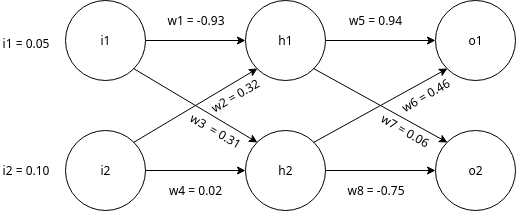
\includegraphics[scale=0.6]{draw-io-backprop-example}
    \caption{Esimerkin neuroverkon syötteet ja painotukset}
    \label{pic:backprop-example}
    \end{figure}

  Lasketaan ensin verkon tuottamat ulostuloarvot syötteillä $i_1 = 0,05$ ja $i_2 = 0,10$ sekä väliltä $[-1, 1]$ arvotuilla painotuksilla $w_1...w_8$. Piilokerroksen neuroneiden syötteiden summaus tehdään kappaleessa \ref{chap:artificial-neuron} esitetyn kaavan $\Sigma x_i w_i$ mukaisesti
  
  $$h_{1}syöte = w_1 * i_1 + w_2 * i_2$$
  $$h_{1}syöte = -0,93 * 0,05 + 0,32 * 0,10 = -0,0145$$
  $$h_{2}syöte = w_3 * i_1 + w_4 * i_2$$
  $$h_{2}syöte = 0,31 * 0,05 + 0,02 * 0,10 = 0,0175$$

  Syöttämällä nämä arvot sigmoidiseen aktivaatiofunktioon saadaan
  $$h_{1}ulos = \frac{1}{1 + e^{-(-0,0145)}} \approx 0,496$$
  $$h_{2}ulos = \frac{1}{1 + e^{-0,0175}} \approx 0,504.$$

  Toistaen vastaavat vaiheet ulostulokerrokselle käyttäen piilokerroksen ulostuloarvoja syötteenä saadaan:
  $$o_{1}syöte = w_5 * h_1 + w_6 * h_2$$
  $$o_{1}syöte = 0,94 * 0,496 + 0,32 * 0,504 \approx 0,628$$
  $$o_{2}syöte = w_7 * h_1 + w_8 * h_2$$
  $$o_{2}syöte = 0,06 * 0,496 + (-0,75) * 0,504 \approx -0,348$$

  $$o_{1}ulos = \frac{1}{1 + e^{-0.627}} \approx 0,652$$
  $$o_{2}ulos = \frac{1}{1 + e^{-(-0.348)}} \approx 0,414.$$

  %Kun harjoitusaineistoksi valitaan arvot $o_1harjoitus = 0.01$ ja $o_2harjoitus = 0.99$ saadaan kaavan \ref{eq:error-function} mukaisesta virhefunktiosta $E(x) = \frac{1}{2} \sum_{i=1}^{N} \| y(x_i)-a(x_i) \|^2$ arvoksi
  Kun harjoitusaineistoksi valitaan arvot $o_{harjoitus1} = 0.01$ ja $o_{harjoitus2} = 0.99$ saadaan kaavan \ref{eq:error-function} mukaisesta virhefunktiosta arvoksi

  $$ 0,5 * ( (0,652 - 0,01)^2 + (0,414 - 0,99)^2 ) = 0,372. $$
  
    \begin{figure}[h]
    \centering
    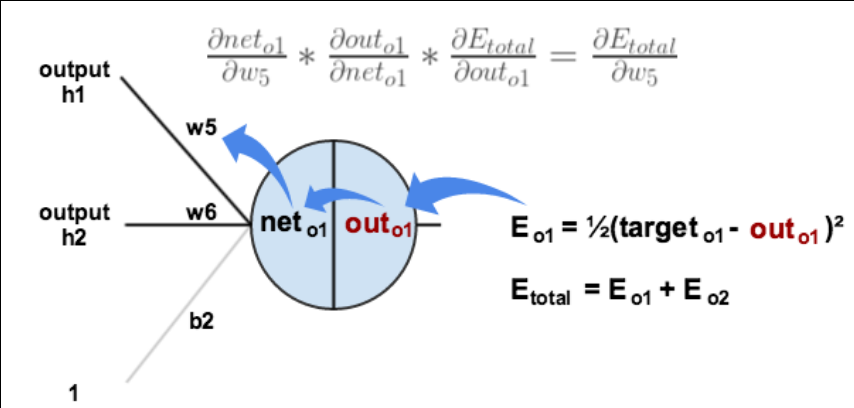
\includegraphics[scale=0.4]{chain-rule}
    \caption{TODO piirrä oma kuva, atm: https://mattmazur.com/2015/03/17/a-step-by-step-backpropagation-example/}
    \label{pic:chain-rule}
    \end{figure}

  Taaksepäinkulkeutumisvaiheessa painon vaikutus koko verkon virheeseen voidaan laskea ketjusäännön avulla

  $$ \frac{\delta E_{koko}}{\delta w_5} = \frac{\delta E_{koko}}{\delta ulos_{o1}} * \frac{\delta ulos_{o1}}{\delta summa_{o1}} * \frac{\delta summa_{o1}}{\delta w_5}. $$

  Lasketaan painon $w_5$ vaikutus virheeseen. $E_{koko}$ koostuu ulostulokerroksen neuroneiden tekemien virheiden summista, joten kun se derivoidaan tietyn neuronin ulostulon suhteen, muiden neuroneiden virheiden termit putoavat pois. Jäljelle jää 
  
  $$ \frac{\delta E_{koko}}{\delta ulos_{o1}} = 2 * \frac{1}{2} (ulos_{o1} - harjoitus_{o1})^{2-1} * 1 = ulos_{o1} - harjoitus_{o1} = 0.652 - 0.01 = 0.651$$

  Sigmoidisen aktivaatiofunktion $ f(x) = \frac{1}{1 + e^{-x}}$ derivaatta on $f'(x) = f(x)(1 - f(x))$.
  Koska $ ulos_{o1} = \frac{1}{1+e^{-net_{o1}}} $ niin

  $$ \frac{\delta ulos_{o1}}{\delta summa_{o1}} = ulos_{o1}(1 - ulos_{o1}) = 0.652(1 - 0.652) \approx 0.227.$$

  $ summa_{o1} = w5 * out_{h1} + w_6 * out_{h2} $ joten viimeinen tarvittava osa 
  $$ \frac{\delta summa_{o1}}{\delta w_5} = 1 * out_{h1} + w_5 * 0 + 0 = out_{h1} $$ 

  joten $\frac{\delta E_{koko}}{\delta w_5} = 0.651 * 0.227 * 0.496 \approx 0.073 $.

  Virhettä korjataan yleensä jonkin oppimistahdin (learning rate) mukaisesti, jota usein muutetaan neuroverkon harjoittamisen aikana. Tässä esimerkissä käytetään mielivaltaisesti valittua $\eta = 0.5$ oppimistahtia. Korjaamme nyt $w_5$ virhettä asettamalla sen uudeksi arvoksi

  $$w_{5}^+ = w_5 - \eta * \frac{\delta E_{koko}}{\delta w_5} = 0.94 - 0.5 * 0.073 = 0.9035.$$

  Muiden ulostulokerroksen neuroneiden syötteiden painotukset voidaan laskea vastaavasti. Piilokerroksen painojen aiheuttaman virheen pienentäminen tehdään muuten vastaavasti, mutta laskettaessa kokonaisvirheen muutosta piilokerroksen neuroneiden ulostuloarvojen suhteen, on otettava huomioon piilokerroksen neuroneiden ulostuloarvojen vaikutus useiden ulostulokerroksen neuroneiden tekemään virheeseen.

  TODO: Pitäisikö laskea neuroverkolle uusi ulostulo kun yksi verkon paino muutettu? Vai laskea kaikille painoille muutokset ja sen jälkeen ulostulo?

  % syötteet: 0.05, 0.10
  % painot: -0.93 0.31 0.32 0.02 0.94 0.06 0.46 -0.75
  % toivotut ulostulot 0.01 0.99


  
  \section{Konvolutionaalisten neuroverkkojen rakenne}
    Konvolutionaalisten neuroverkkojen rakenne eroaa tavanomaisista täysin yhdistetyistä neuroverkoista konvoluutio- ja kokoamiskerroksien (pooling layer), kerrosten mahdollisen rinnakkaisuuden, sekä ominaisuuskarttojen jaettujen painojen kautta.   
    
    \subsection{ReLU}
    ...
    %(TODO:lisää kuvia ja selitystä ytimestä, kuten esitelmähommassa puhuttiin)
    \subsection{Konvoluutiokerrokset}
    
    \begin{figure}[h]
      \centering
      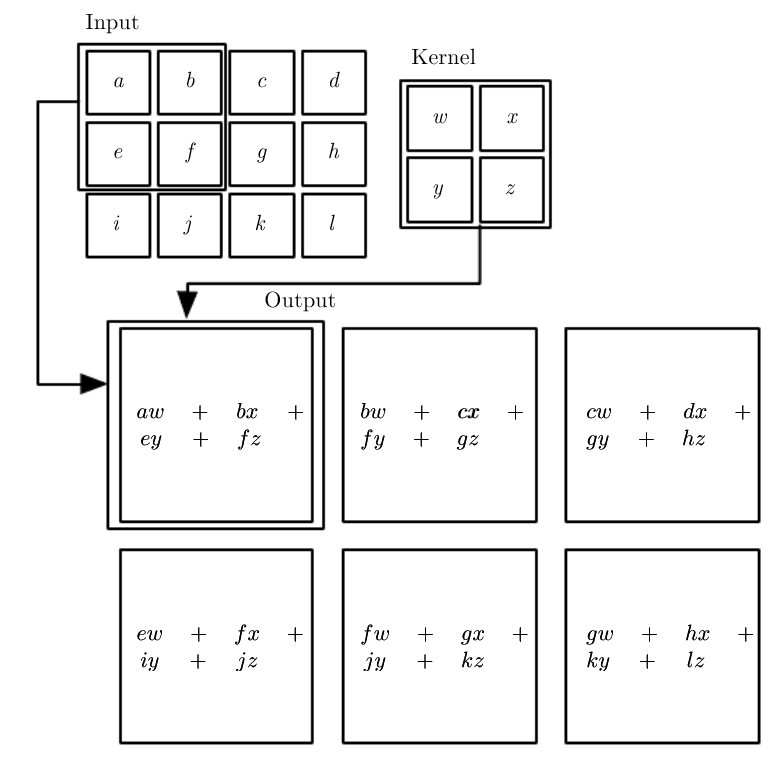
\includegraphics[scale=0.4]{convolution}
      \caption{Konvoluutiokerrosten syötteiden valinta ja ulostulojen muodostuminen \cite{Goodfellow-et-al-2016}}
      \label{pic:convolution}
    \end{figure}

    Konvoluutioverkkojen nimi juontaa juurensa matemaattiseen konvoluutioon, sillä kaava jolla konvoluutiokerrosten neuroneiden syötteet $a_{x,y}$ painotuksineen $w_{x,y}$ voidaan esittää matemaattisesti esimerkiksi 5x5 kokoiselle paikalliselle vastaanottavalle kentälle (local receptive field) muodossa

    % TODO: kuuluuko loppuun pilkku?
    $$ \sum_{l=0}^{4}\sum_{m=0}^{4} w_{l,m}a_{j+l,k+m},$$
    
    joka on käytännössä diskreetti konvoluutio, jossa painotukset ovat konvoluution ydin (kernel).

    Konvoluution voidaan ajatella olevan liukuva ikkuna, joka rajoittaa neuronit saamaan kuvan \ref{pic:convolution} mukaisesti syötteenään vain osan syötekerroksensa ulostuloista, täysin yhdistetyistä neuroverkkokerroksista poiketen. Tämä rajoittuneisuus mahdollistaa neuroneiden erikoistumisen johonkin osa-alueeseen syötteissään, joka on erityisen hyödyllistä haluttaessa käyttää neuroverkkoja syötteiden tutkintaan joissa ilmenee paikallisuutta. Esimerkiksi kuvat ovat erittäin paikallistuneita, pikselien etäisyys toisistaan korreloi vahvasti sen kanssa, liittyykö niiden sisältö toisiinsa.

    Kuvasta \ref{pic:convolution} ilmenee myös toinen yleinen konvoluutiokerrosten piirre: mikäli tehdään vain konvoluutioita joissa ydin mahtuu kokonaan syötekuvaan, konvoluutiokerroksella on vähemmän ulostuloja kuin sisääntuloja. Kuvan tapauksessa nähdään syötematriisin ollessa 3x4, ja ytimen 2x2 kokoinen, ulostulomatriisin kooksi tulee 2x3. Tällä tavalla konvoluutio mahdollistaa myös sen, että konvoluutioverkot voivat ottaa vastaan vaihtelevan kokoisia syötteitä.

    \subsection{Ominaisuuskartat ja jaetut painot}
    % TODO: ei yhtään viitettä
  TODO: lisää kuvia yms. siitä mitä ydin on jne.

  % TODO selitä lisää miten yhteiset painot toimivat
    Konvoluutiokerroksia on yleensä useita rinnakkain, ja konvoluutiokerrosten neuronit jakavat samassa kerroksessa olevien neuroneiden kesken yhteiset painot (shared weights). Kerroksien yhteiset painot mahdollistavat sen, että kukin kerros oppii tunnistamaan translationaalisesti invariantteja ominaisuuksia syötteistään, ja yksittäisen neuronin voidaan ajatella kertovan löytyykö sen saamien syötteiden alueelta tätä ominaisuutta. Esimerkiksi kuvien tapauksessa ominaisuuskartta joka löytää kuvasta suoria viivoja saattaa olla hyödyllinen, sillä suoria viivoja voi ilmetä useassa eri paikassa kuvassa, ja toisaalta korkeammalla abstraktiotasolla kuvassa esiintyvät objektit ovat edelleen sama objekti, vaikka niitä olisi siirretty muutamia pikseleitä johonkin suuntaan.

    \subsection{Kokoaminen ja tehokkuus}
    Usein konvoluutioverkoissa käytetään konvoluutiokerroksien jälkeen kokoamiskerroksia, jotka tekevät yhteenvedon jostakin edeltävästä neuroverkkokerroksen alueesta. Esimerkiksi hyvin yleisen maksimikokoamiskerroksen (max-pooling) neuronit antavat ulostulokseen syöteneuroniensa ulostuloista suurimman.
    %viitteet viitteet viitteet

    Yhdessä kokoamiskerrokset ja jaetut painotukset vähentävät merkittävästi konvolutionaalisten neuroverkkojen harjoitettavien parametrien määrää verrattuna neuroverkkoihin, joissa on vain täysin yhdistettyjä kerroksia. Tällä voidaan nopeuttaa harjoittamista ja lisätä suorituskykyä.

    \subsection{Täysin yhdistetyt kerrokset}
    %TODO: miksi kerrokset haluttaisiin litistää takaisin yhteen?
    Konvoluutiokerrosten kohdalla konvolutionaaliset neuroverkot haarautuvat yleensä rinnakkaisiin kerroksiin. Sijoittamalla verkon viimeiseksi kerrokseksi täysin yhdistetyn kerroksen nämä rinnakkaiset kerrokset voidaan litistää (flattening) takaisin yhteen.

  \section{Konvolutionaaliset neuroverkot käytännössä}
    Konvoluutioverkkoja on käytetty erityisen onnistuneesti kuvien sisällön luokitteluun. Monille kuvia tunnistaville neuroverkoille yhteinen piirre on, että ulostulokerroksessa on yksi neuroni jokaista tunnistettavaa objektiluokkaa kohden, ja neuronin arvo kertoo kuinka todennäköisesti kyseisen luokan objekti löytyy kuvasta.

  \subsection{Verkon toiminnan visualisointi}
  ... \cite{visualizing-convolutional}

  \subsection{Kuvien luokittelu}

    % \subsection{ImageNet kilpailu}
    %   ...

    % ...
    TODO: Imagenet kilpailun kuvailu? Pitäisikö olla oma kokonainen section kuvien luokittelulle ja sen subsectionina imagenet ja CNN:ien toiminnan visualisointi. Esimerkkikuvia imagenet aineistosta?

    \begin{figure}[h]
    \centering
    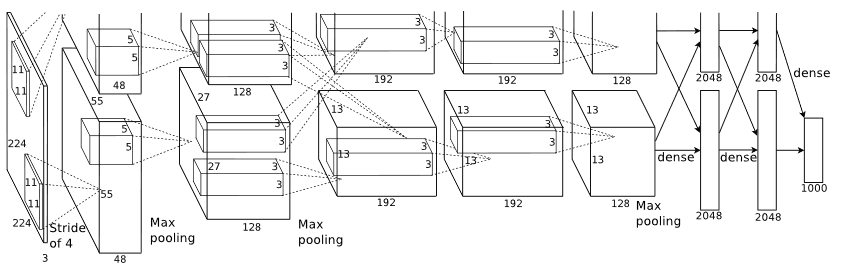
\includegraphics[scale=0.4]{imagenet}
    \caption{ILSVRC-2012 kilpailun voittaneen neuroverkon rakenne \cite{KSHimagenet2012}}
    \label{pic:hsk-neuralnet}
    \end{figure}

    Vuonna 2012 ImageNet kuvantunnistuskilpailun voittaneessa Krizhevsky, Sutskever ja Hintonin (myöhemmin KSH) konvolutionaalisessa neuroverkossa on 7 piilokerrosta, joista 5 ensimmäistä ovat konvoluutiokerroksia, ja 2 viimeistä kerrosta täysin yhdistettyjä kerroksia. KSH:ssa on 1000 neuronin ulostulokerros joka vastaa sen tunnistamaa tuhatta erilaista kuvaluokkaa.
    
    ImageNet kuvamateriaalissa on vaihtelevan kokoisia kuvia, mutta KSH:n luomassa neuroverkon syötekerros oli 3x224x224 neuronin kokoinen. KSH:n ratkaisu syötteen sopivaksi saamiseksi oli skaalata lähdekuvat ensin 256x256 pikselin kokoon, ja tämän jälkeen ottaa kuvista 224x224 osakuvia satunnaisista sijainneista lähdekuvasta, näin laajentaen harjoitusdataa ja vähentäen ylisovitusta.
    
    KSH:n verkossa aktivaatiofunktiona toimi viimeaikoina hyväksi havaittu $R(z) = max(0, z)$ muotoinen Rectified Linear Unitiksi (ReLU) kutsuttu funktio \cite{KSHimagenet2012}.

  \subsection{Jokin muu sovellus kuin kuvien luokittelu?}
  ...
  \subsection{Deep dream}
  Samanlainen toteutustapa kuin takaisinvirtausalgoritmissa, paitsi painotusarvot pysyvät kiinteinä ja muutetaankin syötettä.

  \subsection{Kirjastot}
  Johonkin saisi ehkä pari kappaletta tekstiä (konvolutionaalisten) neuroverkkojen luomista helpottavista kirjastoista yms. kuten TensorFlow.

\section{Yhteenveto} 

Kappale siitä, että sitä ei vielä täysin ymmärretä, miksi neuroverkot oppivat niin hyvin.

Aloitettiin käymällä läpi kaikille neuroverkoille yleisiä piirteitä, kuten yksittäisen neuronin rakennetta ja sitä, miten yksittäisistä neuroneista muodostetaan eteenpäinsyöttävä neuroverkko. Seuraavaksi esiteltiin kuinka neuroverkkoja voidaan harjoittaa harjoitusaineiston perusteella takaisinvirtausalgoritmin ja gradienttimenetelmän avulla. Lopuksi käsiteltiin konvolutionaalisten neuroverkkojen eroavaisuuksia muista neuroverkoista ja esiteltiin käytännön esimerkki konvolutionaalisesta neuroverkosta.

Käsittelemättä jäi (ehkä) miten aktivaatiofunktioita ja muita juttuja valitaan järkevästi/hyvin yms.






  % ------------------------------ References ------------------------------
  %
  % bibtex is used to generate the bibliography. The babplain style
  % will generate numeric references (e.g. [1]) appropriate for theoretical
  % computer science. If you need alphanumeric references (e.g [Tur90]), use
  %
  % \bibliographystyle{babalpha-lf}
  %
  % instead.

  %\nocite{*}
  \bibliographystyle{babplain-fl}
  \bibliography{references}


  % --- Appendices ---

  % uncomment the following

  % \newpage
  % \appendix
  %
  % \section{Esimerkkiliite}

  \end{document}
